\chapter{Background Research}
Migration is a heating topic, attracting increasing people to figure out what strategies behind. The project is all about prisoner's dilemma and spatial movement, thus many papers about game theory are gone through and can be classified as four categories: game theory, spatial games, migration games and experiments on migration. In this section, they will be reviewed respectively and probably may provide an overall idea of how this project comes and what techniques are used.
\section{Game Theory}
\subsection{Classic Game Theory}
As \citet{myerson2013game} mentions, game theory can be defined as a multi-disciplinary study providing general mathematical models of looking for optimal strategies for a game which exists conflict and cooperation between rational decision-makers and of analysing scenarios that one individual's choice will affect on another's payoff. At first, game theory was utilised in a branch of applied mathematics. Later, however, it was used for solving social problems in various fields such as physics, ecology, economics, computer science and so on.

"Game" is the abstract concept in game theory that it is a scenario for decision-makers, also known as "players", to find their most beneficial strategies. Every game contains a matrix which describes different combinations of decisions and relevant welfare and normally, it is a $2 \times 2$ table. It is assumed that all players are selfish who always care about themselves and try to maximise their own expected payoff. The "payoff" is determined by the player's strategy and others' choice. In game theory, "solution" is a strategy and result that a player can use to maximise bonus. According to \citet{cremer1988full}, a dominant strategy is considered as a competing strategy that no matter what others choose, it is the best strategy for the player itself.

A milestone of game theory is the solution of Nash Equilibria which was put forward by John Nash in  1950s \citep{nash1951non}. A Nash Equilibria is applied to solve non-cooperative game and it is a set of strategies in which combination no one could increase payoff by deviating so no player has an incentive to individually change strategy. Nash Equilibria can be categarised as \textit{pure} strategy Nash Equilibrium and  \textit{mixed} Nash Equilibrium. Pure Nash Equilibrium is the best strategy for players on the assumption of complete description of decisions that rational players will make is known. In the game of stag hunt which can be illustrated as \tref{Table:tabex}, the Nash Equilibrium point is to cooperate to hunt stag together.

\begin{table}[!htb]
  \centering
  \begin{tabular}{c | c | c}
  \toprule
  \textbf{} & \textbf{Stag} & \textbf{Hare}\\
  \midrule
  \textbf{Stag} & 2,2 & 0,1\\
  \midrule
  \textbf{Hare} & 1,0 & 1,1\\
  \bottomrule
  \end{tabular}
  \caption{Stag hunt example. This scenario describes two hunters want to hunt stags together. One of strategies should be picked and payoff depends on different combinations. If both players choose to cooperate to hunt stag, they will get the most bonus. If one cooperates but the other defects, the defector will acquire more award than the cooperator. If both of them defect, they will get bonus but less than cooperating together.}
  \label{Table:tabex}
\end{table}

Games can have and not have multiple Nash Equilibrium points. Even if it exists, it can also not be the best strategy. Therefore, there is mixed Nash Equilibrium which defines a strategy with some probability of playing each pure strategy, providing different response to a player in an identical scenario. A classic example of mixed Nash Equilibrium is pennies game which is also a zero-sum game. Both players play each strategy with equal probability of mixed Nash Equilibrium which means they had better play randomly.

\subsection{Prisoner's Dilemma}
Prisoner's dilemma is known as a classic situation of social dilemma. It is always used to model social situation that exists cooperation and defection. Two criminals are arrested  but the police do not have enough proof of their crimes, thus they are detained separately and questioned individually. The police give them two choice: confession or denial. If they both deny, they will be sentenced for half a year because of lack of evidence. If both of the confess, which means they cooperate with each other, then they will be detained for two years. However, if one confess but the other deny, the one confess will be released right now, while the other should be put in prison for ten years. For a more formal definition, the payoff matrix can be described in \tref{Table:pdmatrix}. In prisoner's dilemma, it is assigned values as $T > R > P > S$ and $2R > T + S$, which is more profitable to defect. Therefore, it is higher possible to defect when players meet once.

\begin{table}[!htb]
  \centering
  \begin{tabular}{ c | c | c }
  \toprule
  \textbf{} & \textbf{C} & \textbf{D}\\
  \midrule
  \textbf{C} & R,R & S,T\\
  \midrule
  \textbf{D} & T,S & P,P\\
  \bottomrule
  \end{tabular}
  \caption{Matrix of prisoner's dilemma. A player should choose 'C' or 'D' and could receive payoff. In the matrix, R is "reward" for mutual cooperation \citep{helbing2009outbreak} whereas "punishment" P is bonus for defection on both sides. When there is unilateral defection, "sucker's payoff" S is for the cooperating and "temptation" T is for the defector. }
  \label{Table:pdmatrix}
\end{table}

The prisoners cannot communicate with each other, so they have to independently look for an optimal strategy. Take the column for example. If the row player confesses, confession as well is the best for him to receive less sentence ($T > R$). On the other hand, if the other stays silent, it is best to testify against him as the inequality $P > S$, then he can be released. Therefore, confession all the time can receive the least payout no matter what is chosen by the other person. This is known as a dominant strategy, an action always returns the highest payoff regardless of the other's choice. It is also a Nash Equilibrium, but if both attempt to testify, it is not the best strategy combination as can be observed in the matrix. A conclusion can be made here: Nash Equilibrium sometimes can be a suboptimal solution.

If the inequalities given previously is changed a bit to $T > R > S > P$, it becomes snowdrift game which encourages more to cooperate \citep{hauert2004spatial}. Or if change it to $R > T > P > S$, it is the stag-hunt game in which scenario if both defects, they can receive a small payoff instead of severe punishment. According to \citet{perc2010coevolutionary}, compared with the prisoner's dilemma, the stag-hunt game incents more to cooperate in that the payoff for mutual cooperation is higher than temptation of defection. The prisoner's dilemma, however, is considered offering the strongest support for selfish behaviour.

The classic prisoner's dilemma game soon confronted its limitation upon the assumption of settings that the two same individual will meet more than once and they can remember what the other's previous action and payoff. This becomes an iterated prisoner's dilemma \citep{axelrod1987evolution}. There are two mainstream "winning strategies" - \textit{"tit for tat" and "win-stay, lose-shift"}. \citet{axelrod2006evolution} held two tournaments and found that "tit for tat" is the simplest but steady solution. This strategy always starts with a cooperative choice and repeats what the other player does in the last round. It does not always win in the repeated prisoner's game, but anyway, if it loses, it will not lose much. In addition, when it encounters the same "tit for tat" solution, they will keep cooperating to maintain the status. Soon researchers found "tit for tat" cannot correct mistakes caused by noise and eventually, it was replaced by "win-stay, lose-shift" which is even a simpler solution, repeating previous move if you win until you lose, then changing to the other strategy \citep{nowak1993strategy}. As \citet{nowak2006five} writes in "Five Rules for the Evolution of Cooperation", if cooperative society has been established, win-stay, lose-shift is more possible to maintain it.

\subsection{Evolutionary Game Theory}
Aforementioned introduction of game theory is the game played just once by rational players who know all detail of the game. In reality, however, development of society is a long-run aggregate behaviours. For instance, a small difference of gene can be a factor leading an animal survive and as time goes, it is enlarged, even resulting in natural selection. The similar question is raised in the field of economics. A small policy decision can have a large effect on the future situation in such a fierce market competition. How to estimate the outcome if the game is played over and over again attracts a wide range of research and recent research mostly focuses on models of abstract social scenarios of evolutionary games.

Evolution was first explicitly applied in game theory in 1961 \citep{smith1982evolution}. At that time, it was used to model species playing games against nature and looking for strategies to minimise the probability of extinction. "The Evolution of Cooperation" \citep{axelrod2006evolution} built a bridge to economics and social science. As it mentions, evolutionary game theory is an extension of classical game theory, solving the problem to determine strategies when the fitnesses (payoffs) rely on the relative possibility in the population of all phenotypes (strategies) involved. The aim of evolutionary game theory is to remedy three main shortages of classic game theory: (1) bounded rationality, (2) the lack of dynamics, and (3) equilibrium selection in the case of multiple Nash equilibria \citep{szabo2007evolutionary}. Here, compared with features in prisoner's dilemma, the player has a fixed strategy instead of being required to have a rational strategy.

A large population is definitely probable to cause uncertainty, thus a crucial problem of evolutionary game theory is to make the population stable and robust enough for strategy profiles. To discuss stability, there is another notion named "game dynamics" which is defined by \citep{taylor1978evolutionary}, as the equation shown below:

\begin{equation}\label{eq:2.1}
    \dot{s_i} = s_i [ F(i|s) - F(s|s)].
\end{equation}

where $s_i=n_i/N$ is the proportion of \textit{i}-strategies, and the state or distribution of strategies of population is the vector $s=(s_1, \ldots, s_n)$. $F(i|s)$ is the fitness of a strategy with a growth rate $r_i$ and $F(s|s)$ represents the average of fitness. The equation describes how to determine the strategy in a specific state, taking into account the current growth rate and the average payoffs.

Furthermore, evolurionary dynamics are studied by replicator equation, showing in \eref{eq:2.2}, which assumes a uniform population distribution. In reality, it is observable that continuous form can be obtained from the discrete form. In the equation, $x_i$ is the percentage of \textit{i}-strategy in the population and $A$ is the fitness information like a matrix. The expected payoff for an individual of type \textit{i} is written as $(Ax)_i$ and the average fitness of the population as a whole is $x^TAx$ in the equation.
\begin{equation}\label{eq:2.2}
    \dot{x_i}=x_i\left(\left(Ax\right)_i-x^TAx\right).
\end{equation}

 The first solution was raised by \citet{smith1973lhe} in 1973 - Evolutionarily Stable Strategy (ESS) which can be defined as a strategy that is uninvadable by a minority of mutant strategy that would gain higher fitness, when it is used by the majority of the population. Players who adopt ESS have a better performance than mutants and outcompete in a long-run period, eventually it turns out expelling invaders and the stable state in the population arises. This persists as a dominant strategy in the whole evolutionary procedure. It can be observed that many phenomena in the society use ESS.

\section{Spatial Games}
Spatial Game is an extension of evolutionary social dilemma which defines a lattice, allowing population in the map to play a game of a specific scenario over and over again and it is used to analyse different strategies by modeling an evolutionary game. In spatial games, cooperation is a crucial problem to solve.
\subsection{Cooperation in Spatial Games}
\citet{dawkins2006selfish} states in the book that every gene, every cell and every organism should be selfish in a fierce competition of environment to outcompete its competitors so that they could promote its own evolutionary success. However, cooperation is an objective existence in our society which is thought to be conflicting against natural selection.  It means "selfish  replicators forgo some of their reproductive potential to help on another", as defined by \citet{nowak2006five}. A cooperator of a game is someone who plays a strategy of  collective reality and it can have two results: (1) if the other player has the same decision, they both receive reward "R"; (2) if the other betrays, a sucker's payoff "P" which is always less than the defector's fitness will be received. Compared with a population of only defectors which has the lowest fitness, a population of only cooperators has the highest average fitness. However, as can be seen in \fref{Figure:figns}, it suggests average fitness is constantly reducing because a selfish defector could always get higher mean fitness, so defection can be more possible to happen in spatial game.
\begin{figure}[!htb]
  \centering
  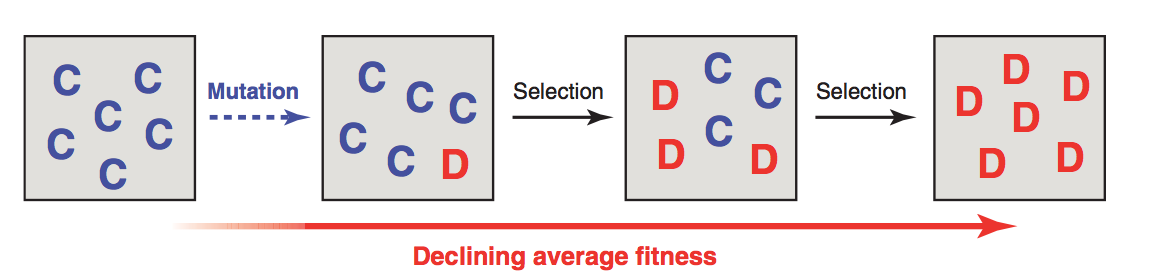
\includegraphics[width=12cm]{figns.png}
  \caption[Natural selection favors defectors]{Natural selection favors defectors \citep{nowak2006five}}
  \label{Figure:figns}
\end{figure}

\subsubsection{Kin Selection}
Kin selection is defined as a rule that cooperative behaviours can have beneficial effect on individuals who have the shared gene. This is reasonable that species carrying similar gene can increase their fitness by cooperation, thus it is supported by natural selection and considered as the consequence of "selfish genes". As it encourages players constantly remain cooperation, it is convinced that the highest fitness will be received. This rule, however, has limitation which is just applied to cooperation between relatives or those have similar strategies.
\subsubsection{Direct Reciprocity}
To explain cooperation between two different species, another mechanism, direct reciprocity, was proposed by \citet{trivers1971evolution} in 1971. He defines it as a new rule for cooperative behaviours between individuals who are not closely related. To be specific, it is assumed that two player can meet again and they can choose cooperation or defection in every round, knowing each other's previous strategy and being able to provide help. Two popular winning solution for playing this game is \textit{tit-for-tat} and \textit{win-stay, lose-shift}. Tit-for-tat is to choose the strategy of what the other has chosen in the previous round which has a satisfactory performance but could not correct mistakes, leading to a continuous retaliation. Win-stay,lose-shift strategy can solve this problem and it is an idea that hold the move when winning and change when you lose. 

If the probability to meet the same players, $w$, is greater than the benefit $b$ to cost $c$ of the altruistic act, direct reciprocity allows evolution of cooperation, as given by \eref{eq:2.3}:
\begin{equation}\label{eq:2.3}
    w > c/b
\end{equation}
\subsubsection{Indirect Reciprocity}
Unselfish behaviours between different individuals in indirect way also can be observed in society. For instance, one person donates to charity but not to direct recipients. In this way, interaction is not symmetric that means it may just has one direction which is different from mutually straight interaction of direct reciprocity (\fref{Figure:figdf}). This type of reciprocity introduces the concept of reputation which is able to be used to form friendship networks. According to \citet{milinski2002reputation}, indirect reciprocity based on reputation can sustain a high level of cooperation, but if there is unexpected indirect reciprocity, fitness will drop rapidly down to zero. On the other hand, reputation can result in higher profits for all players. Although indirect reciprocity is rarely found in nature, it is highly believed helpful to form moral system in human society.

\begin{figure}[!htb]
  \centering
  \subfigure[Direct reciprocity]{
  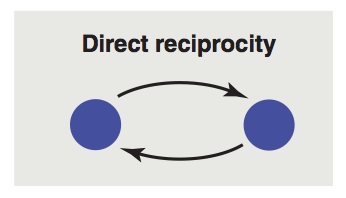
\includegraphics[width=5cm]{dr.png}
  \label{Figure:sfig1}
  }
	\quad
	  \subfigure[Indirect reciprocity]{
	  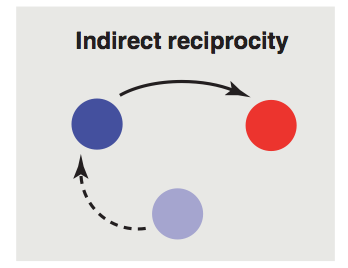
\includegraphics[width=5cm]{indr.png}
	  \label{Fiture:sfig2}
	  }
  \caption[Two mechanisms for evolution of cooperation]{Two mechanisms for evolution of cooperation \citep{nowak2006five}}
  \label{Figure:figdf}
\end{figure}

\subsubsection{Network Reciprocity}
It is common that natural selection is based on unwell-mixed population, where mutual interaction is not equal among individuals. Network reciprocity focus on frequency of interaction of population, assuming populations are not well mixed. \citet{nowak1992evolutionary} argues that without any strategic complexity, forming network clusters where cooperators can assist each other is helpful for cooperators to outcompete.

Network reciprocity can only promote cooperation if the benefit-to-cost ratio exceeds the average number of neighbours, $k$ ,which can be seen as the following equation:
\begin{equation}\label{eq:2.4}
    b/c > k
\end{equation}
\subsubsection{Group Selection}
Group selection is defined as a selection that individuals are formed as a group and suggests that groups with a higher lever of cooperation will defeat those with lower. \citet{traulsen2006evolution} built a model of multilevel selection as follows. A population is subdivided into groups where cooperators help each other but defectors do not. Members of a group determine their strategy based on fitness in an evolutionary game. Gradually, offspring are added to the same group, resulting in enlargement of individuals with similar strategy. If a group reaches a certain size, it will split into two. Division continues in those groups with faster reproduction. Then competition between groups emerge because of different speed of group growth. In particular, defection happens more within a group than collective behaviours does, whereas pure cooperator groups grow faster than pure defector groups. That means selection is different in multiple levels - on the lower level, it is more likely to defect, but on the higher level selection favours cooperators.

Mathematically, in order to favour cooperation, the relation between the benefit-to-cost proportion and the ratio of the maximum group size $n$ to number of groups $m$ should satisfy the condition as follows:
\begin{equation}\label{eq:2.5}
    b/c > 1+ (n/m)
\end{equation}
\subsection{Spatial Prisoner's Dilemma Game}
Prisoner's dilemma game, which was clearly introduced in the previous section, has been studied to look for optimal strategy for conflict between selfish individuals and altruistic behaviour. Generally, spatial prisoner's game is assumed that an individual can interact with four immediate neighbours, deciding either cooperation or defection.Total payoff depends on each two players' strategy combination in which has been defined in the so-called payoff matrix. Recent research has concentrated on modelling spatial prisoner's dilemma game.

 \citet{nowak1992evolutionary} introduces a two-dimensional spatial game as follows. Prisoner's dilemma is applied as a basic fitness matrix, only considering two strategies - cooperation and defection. Every player plays against the nearest neighbours in each round and the winner who receives the highest payoff will occupy the site. Afterwards, a second round starts as the previous rules and it may iterate for finite times. Without remembering players or strategies, this model can generate a spatial pattern that contains indefinite collective and treacherous behaviours. Eventually, it is found that introduction of spatial structure can promote formation and maintainance of cooperative clusters to resist invasion from defectors. Interestingly, they found sequence of evolutionary spatial prisoner's dilemma game can be extremely beautiful which can be seen in \fref{Figure:wanhuatong}.
 \begin{figure}[!htb]
  \centering
  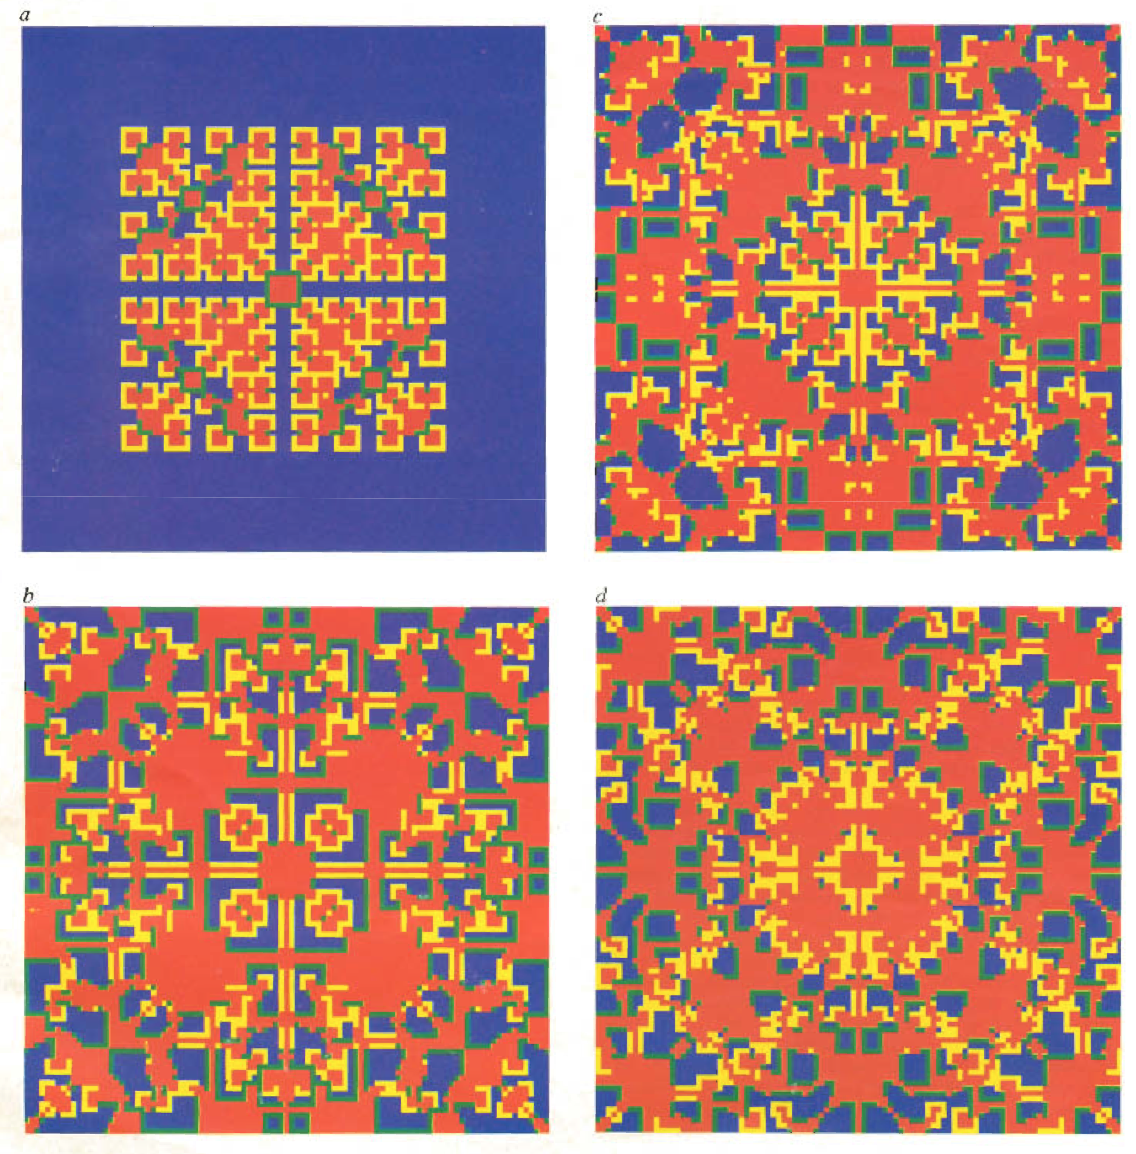
\includegraphics[width=8cm]{wanhuatong.png}
  \caption[Evolutionary kaleidoscope generated by spatial games]{Evolutionary kaleidoscope generated by spatial games \citep{nowak1992evolutionary}. Blue represents cooperation which cooperated in the previous game and red is defection following the same strategy. Yellow is defection following cooperation, while green describes cooperation following defection.}
  \label{Figure:wanhuatong}
\end{figure}

In addition, there are some other models relating to prisoner's dilemma game on a square lattice. A new model is created by \citet{szabo1998evolutionary}. Specifically, the fitness matrix is created as  \citet{nowak1993spatial} suggest, "reward" R=1, "punishment" P=0, "sucker's payoff" S=0 and "temptation" T=b where $b>1$. Therefore, what a defector can get most is $4b$ whereas a cooperator can receive 5 totally if the surroundings are all cooperators. In this model, a randomly picked player has a probability to adopt the neighbour's strategy which can be shown as \eref{eq:2.6}
\begin{equation}\label{eq:2.6}
   W=\frac{1}{1+exp[-(E_Y-E_X)/K]}
\end{equation}
where $E_X$ and $E_Y$ denote total payoffs of player X and Y, respectively and $K$ is the noise allowing irrational decisions. This game will be played for finite time.

\section{Migration Games}
\subsection{Neighbourhood structure}
\subsubsection{Static Neighbourhoods}
Static neighbourhood structure assumes all players are categarised in different groups and individuals in the same group will not change to another group. For example, players who play a specific video games, especially multiplayer online battle arena, can be divided into a grandmaster, a national master, a professional or an amateur. Generally, grandmasters play among themselves, professional players play with those professional and so on. Professional people will upgrade to grandmasters or degrade to an amateur. According to \citet{lecturePPT}, there is a theorem: \textit{let G be a neighbourhood graph and let m be the number of neighbourhoods (cliques) and let M be the maximum size of a clique. If all the players are of the same type t then the game stabilises in at most $mM$ steps.} In this theorem, type $t$ can be defined as follows: if the payoff in round $K$ is greater than 0.5, then play with the same action. If all players use a different strategy, then change to this strategy in the next round. In this case, it is similar to the "win-stay, lose-shift" solution.
\subsubsection{Dynamic Neighbourhoods}
Dynamic neighbourhood structure allows players move between groups. In the model given by \citet{lecturePPT}, players change to the neighbour's group when the neighbour's payoff is greater than his, otherwise stay the same. To make the population stable, it should take $n^{n(n+1)/2}$ steps at most.

To make the definition of dynamic neighbourhoods clearer, an example can be described like a vegetable seller with pushcarts in the market \citep{paul2011neighbourhood}. First of all, the location can dynamically changed according to the demand of this neighbourhood, who sells around and how well other sellers do. Moreover, product is flexible based on different preferences in the neighbourhood and determined by a complex rationale. Finally, the price varies depending on general market situation. If selling in a poor community, the price should be affordable for citizens there. In this instance, location modification can be thought as change between groups and others represent the player's strategy which can be determined in many aspects by how much payoff can be received.
\subsection{Experiments on Migration Games}
In the paper of \citet{helbing2009outbreak}, success-driven migration is proposed that it can promote cooperation in a spatial game. In prisoner's dilemma game, clusters of cooperators can get the most payoff which means if all cooperators stay together without defectors, fitness will maximise. Therefore, in Helbing and Yu's model, cooperators leave the neighbourhood which contains a defector and look for more favorable ones and remain in cooperative neighbourhood. In this case, it satisfies with ESS which can form cooperative population and it is immune to defection.










